\chapter{}\label{ex:aufg4}

\section{}\label{sec:aufg4a}
Der Stromverlauf in einer Wicklung wird in Abb. \ref{fig:stromdelle_Vollschritt} beim Vollschritt dargestellt.


\section{}\label{sec:aufg4b}
Die erkennbare Delle im Stromverlauf in Abb. \ref{fig:stromdelle_Vollschritt} und \ref{fig:stromdelle_Halbschritt} rührt daher, dass durch die Bewegung des Rotors eine Spannung induziert wird, die der Strangspannung entgegenwirkt. Den PT1-Förmigen Verlauf von Abb. \ref{fig:stromdelle_manuell} kann erreicht werden, indem die Stellung angefahren wird, an der sich der Rotor nicht bewegt wenn die Spannung eingeschaltet wird.
\begin{figure}[htb]
	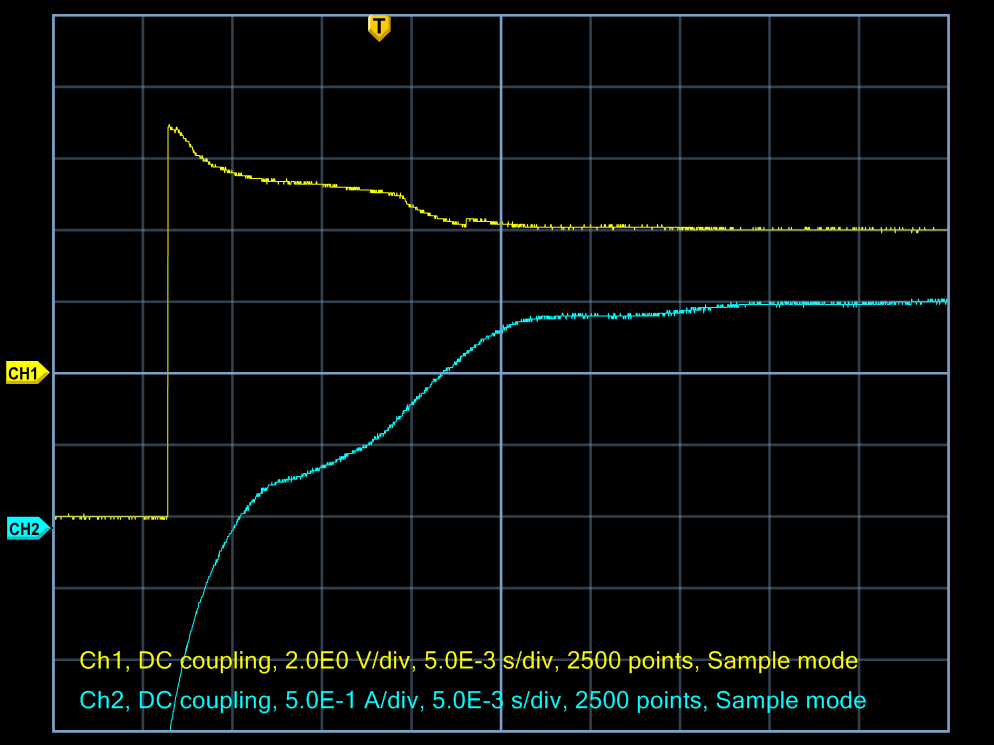
\includegraphics[width=\textwidth]{./Bilder/aufg4_Vollschritt_Stromdelle_1}
	\caption{Stromdelle beim Vollschritt}
	\label{fig:stromdelle_Vollschritt}
\end{figure}
\begin{figure}[htb]
	\centering
	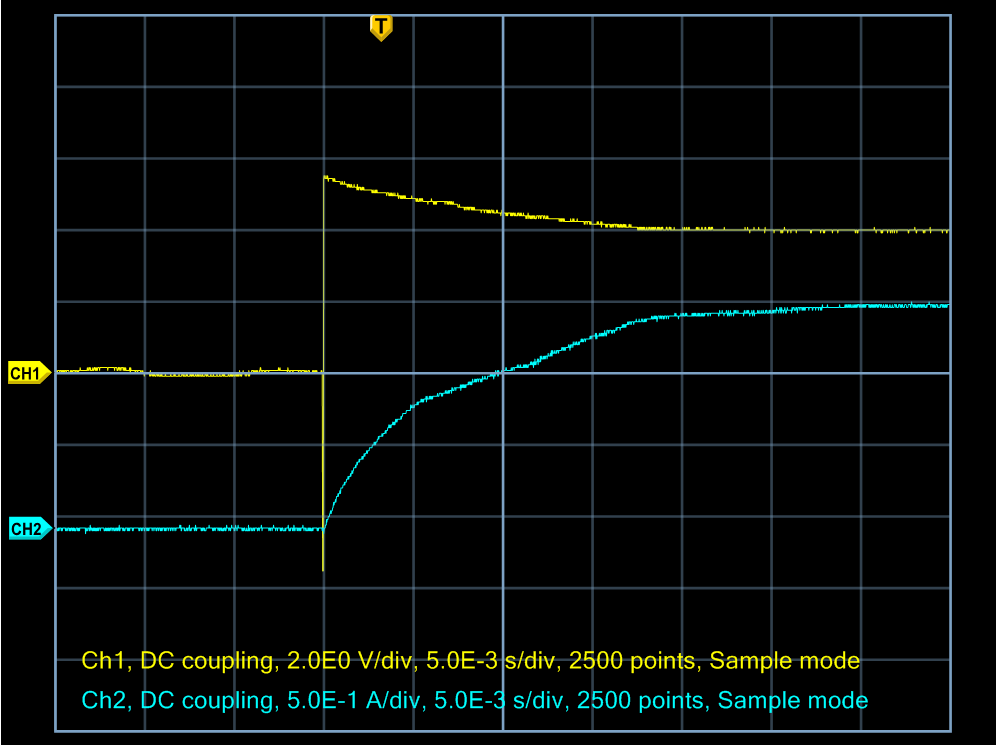
\includegraphics[width=0.8\textwidth]{./Bilder/aufg4_Halbschritt_Stromdelle_1}
	\caption{Stromdelle beim Vollschritt}
	\label{fig:stromdelle_Halbschritt}
\end{figure}
\begin{figure}[htb]
		\centering
	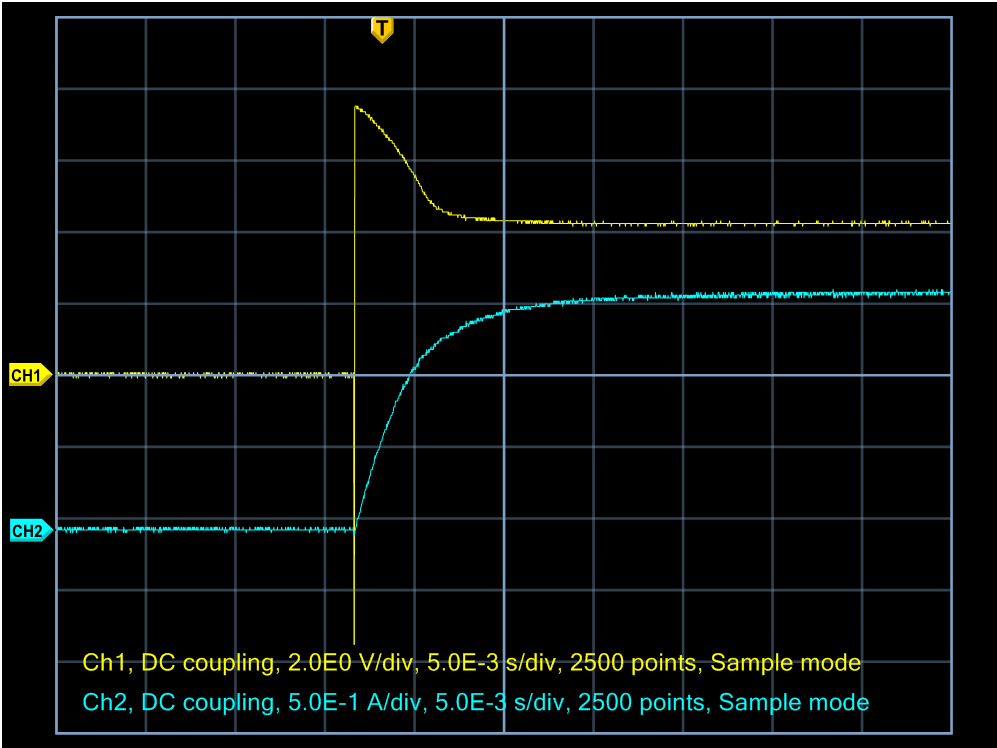
\includegraphics[width=0.8\textwidth]{./Bilder/aufg4_manuell_ohne_Stromdelle_1}
	\caption{Stromdelle ausgeglichen durch manuelle Bestromung}
	\label{fig:stromdelle_manuell}
\end{figure}

\clearpage